% !TEX spellcheck = en_US
%=================================================================================
\chapter{Controller tuning}

In this chapter first calculated the steady-state value to initialize the simulation. After that, the focus to DEL calculation and parameter optimization, minimum pitch angle and the minimum pitch angle optimization for control region 1.5.


%=================================================================================
\section{Steady States (Soni)} \label{steady states}
% !TEX spellcheck = en_US

The steady states are influenced by the design of the controller and turbine.
The static behavior in every operating point can be shown by the calculation of steady states.
Such calculated steady states provide an crucial overview of the turbines behavior early in the design process.
Additionally, these steady states play an important role in the overall wind turbine design and can be utilized to initialize simulations.

The general procedure we followed to find the steady state parameters is as follows: 
\begin{enumerate}
	\item Determine the wind speeds for the control regions. 
	\item Calculate the steady states below the rated wind speed separately for regions 1, 1.5, 2, and 2.5. With the determined wind speeds from step 1.
	\item Calculate the steady states above the rated wind speed.
\end{enumerate}

With the help of the differential equation \ref{eq:omega dot} for the rotor motion the steady states are derived.

\begin{equation}
	\dot{\Omega} = \frac{M_a(v_0, \Omega, \theta) - M_G}{J}
	\label{eq:omega dot}
\end{equation}

The condition to reach a steady state is $\dot{\Omega} = 0$. The determined parameter is the variable and the other parameters are fixed. The conditions to which the fixed parameters are set depending on the control region hence the behavior of the turbine itself.

%Find $v_{rated}$, $v_{1to1.5}$, $v_{1.5to2}$ and $v_{2to2.5}$ using the minimization problem method, as shown in \ref{equation:Minimization problem}. 
%Additionally, use the minimization problem method to determine the above-rated wind speed, as shown in Equation \ref{equation:Minimization problem above rated wind}.
%
%\begin{equation}
%	\min_{v_0} \left( M_a(v_0, \Omega, \theta) - M_G \right)^2
%	\label{equation:Minimization problem}
%\end{equation}
%
%
%\begin{equation}
%	\min_{\theta} \left( M_a(v_0, \Omega, \theta) - M_G \right)^2
%	\label{equation:Minimization problem above rated wind}
%\end{equation}

In the \gls{shakti} model, simulations are performed for wind speeds ranging from 3 to 25 m/s.
The steady state values for wind speed, pitch angle, rotor speed, tip speed ratio, power coefficient, generator torque and tower top displacement are derived by \ref{eq:omega dot}.
Additionally, the results are visually assessed through plots.
The wind speeds of the control regions are $v_{rated} = 9.3531$, $v_{1to1.5} = 6.0652$, $v_{1.5to2} = 6.0652$ and $v_{2to2.5} = 8.6631$. Figure \ref{fig:power cureve} demonstrates the model's power curve.

\begin{figure}[h]
	\centering
	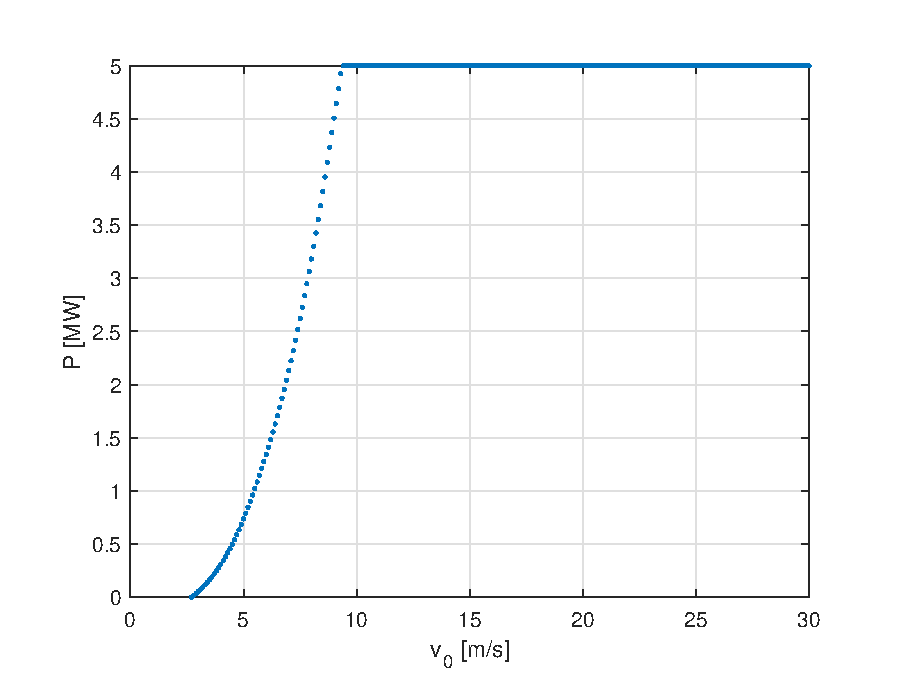
\includegraphics[width=0.7\textwidth]{Figures/P_Vs_v.eps}
	\caption{Power curve calculated with steady state calculations}
	\label{fig:power cureve} 
\end{figure}


\section{DEL calculations and Parameter Optimization (Felix)} \label{DLC 1.2 tuning}
% !TEX spellcheck = en_US
% Parameter Optimization
%=================================================================================
To optimize the controller and its parameters such as $k$ in Control-Region 2, $kp$ for the pitch control in Control-Region 3, $\Delta P$ in  Control-Region 2.5 and $\theta_k$ in Control-Region 3, a brute-force optimization pattern has been followed.

The used method runs the \gls{DLC} 1.2 for the selected control parameter for a specified range of the control value. 
Used wind disturbance is created beforehand with the use of \textbf{TurbSim} and the \textit{GenerateTurbSimWindFields.m} file from the \textit{LAC SummerGames 2024} \cite{SummerGames}. 
The following input parameters to \textbf{TurbSim} have been changed: The turbulence class is set to \textit{B} and the wind-field-grid values are set to match the dimensions of the \gls{shakti}. 
The wind time series are created in a range of $[4:2:24]\frac{m}{s}$ with $6$ different seeds per wind speed. 
The length of the series are $T = \SI{600}{s}$. 
In the \gls{DLC} calculation the simulation is done $6$ times per wind speed for all different seeds. And for all $12$ wind speeds. The total simulation time per wind speed ads up to $T_{\text{Simulation}} = \SI{3600}{s}$. 
With this setup the over speed, life time weighted \gls{DEL} and the \gls{AEP} is computed. 
The used Weibull parameter for the lifetime weighting are $C = \frac{2}{\sqrt{\pi}}\cdot7.5$, this corresponds to the wind class \MakeUppercase{\romannumeral 3} \cite{IEC61400-1} and a $k = 2$. 
\ref{eq:Weibull} shows how the Weibull distribution is computed in this case.
\begin{equation}
	f(V_{\text{ref}}) = \frac{k}{C}\left(\frac{V_{\text{ref}}}{C}\right)^{k-1} \exp\left(-\left(\frac{V_{\text{ref}}}{C}\right)^k\right)
	\label{eq:Weibull}
\end{equation}
The weighting function is derived to \ref{eq:Weighting}
\begin{equation}
	w(V_{\text{ref}}) = \frac{f(V_{\text{ref}})}{\sum f(V_{\text{ref}})}
	\label{eq:Weighting}
\end{equation}
The \gls{AEP} is calculated as \ref{eq:AEP}
\begin{equation}
	AEP = \sum \left(\bar{P}_{\text{el}}w(V_{\text{ref}})\right)\cdot \SI{8760}{h}
	\label{eq:AEP}
\end{equation}
The DEL calculation is using the parameters of the Woehler exponent as $m = 4$ hence this is the typical value for steel a reference number of $N_{\text{ref}} = \frac{2\cdot10^6}{20\cdot8760}$ as a value for 20 years for 1 hour simulations.
The \gls{DEL} is calculated per $V_{\text{ref}}$ with the use of the rainflow count as $\text{DEL}(V_{\text{ref}})$ and the life time weighted \gls{DEL} is than calculated in \ref{eq:LTW-DEL}.
\begin{equation}
	\text{DEL}_{\text{LTW}} = \left(w(V_{\text{ref}})\text{DEL}(V_{\text{ref}})^m\right)^{\frac{1}{m}} 
	\label{eq:LTW-DEL}
\end{equation}
The parameters $\Delta P$ in Control-Region 2.5 and  $k$ in Control-Region 2 are optimized first hence they are not depending on another control parameter. Figure \ref{fig:DeltaP} shows one example of how the optimization results are displayed. The chosen control parameter is $\Delta P = \SI{4.9}{MW}$ hence the \gls{AEP} is higher than for $\Delta P = \SI{5}{MW}$ without a change in the life time weighted \gls{DEL}.
\begin{figure}[h]
	\centering	
	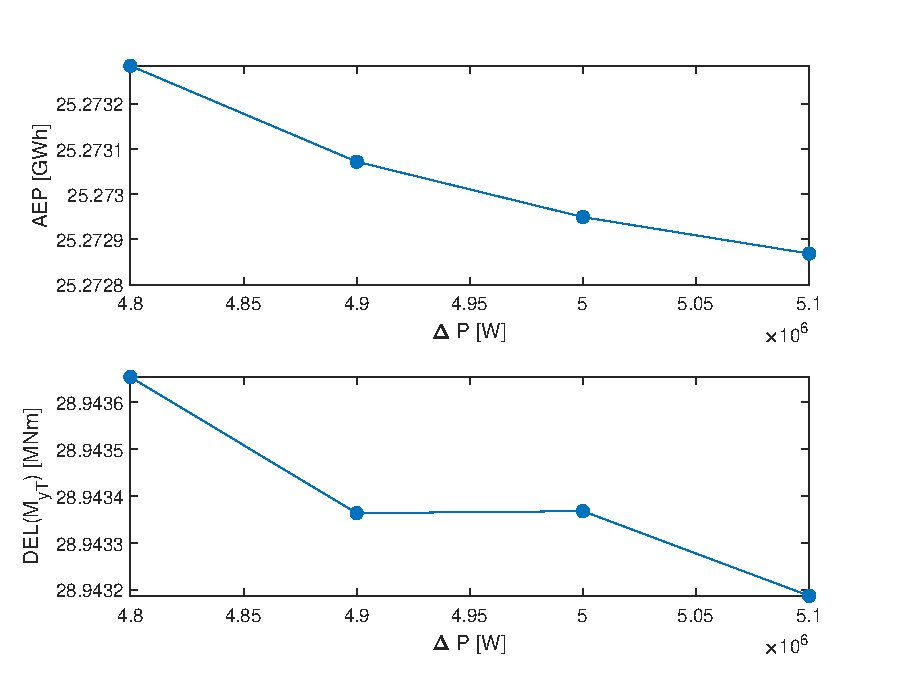
\includegraphics[width=12cm]{Figures/DeltaPopt.eps}
	\caption{Brute-Force optimization of $\Delta P$}
	\label{fig:DeltaP}
\end{figure}

The design value of $k$ is derived first with the help of \ref{eq:k} based on \cite{SchlipfLecture}.
\begin{equation}
	k = \frac{1}{2}\rho\pi R^5 \frac{c_{\text{P,opt}}}{\lambda_{\text{opt}}^3 r_{\text{GB}}^3}
	\label{eq:k}
\end{equation}
The value out of \ref{eq:k} is $k_{\text{design}} = \SI{46.3035}{Nm/(rad/s)^2}$. This is than brute force optimized with a step size of 0.1 as described above.
The resulting value $k$ can next to the other optimized parameters be found in \ref{Control Parameters}. 

The \gls{cpc} gain $kp$ and the gain scheduling parameter $\theta_k$ are effecting not only the \gls{AEP} and the \gls{DEL} of the tower but also the over speed. This introduces another optimization layer. The over speed is computed as \ref{eq:overspeed}. 
\begin{equation}
	\overset{+}{\Omega} = \frac{\hat{\Omega}}{\Omega_{\textnormal{rated}}}
	\label{eq:overspeed}
\end{equation}  
Due to the late design freeze the final \gls{shakti} design leads to low over speeds (less then 10\%). 
A new iterative optimization needs to be done in the future.
The current values are all listed in \ref{Control Parameters}.

\section{Minimum Pitch Angle Optimization (Julius)} \label{minimum pitch angle static}
% !TEX spellcheck = en_US
% Theta min static calculations
%=================================================================================
The optimization of the minimum pitch angle is a simple adjustment which leads to a small increase in the AEP. 
The optimization was done with a brute force approach and the steady states calculations (Section \ref{steady states}). 
In control region 2 the WT should work at optimum $Cp$ and $\lambda$. 
The use of minimum pitch angle can lead to an more efficient state of the turbine at the start of region 2 and therefor increase the AEP. 
For different pitch angles the steady states where calculated. 
As optimum, min. pitch angle the angle which leads to the highest $Cp$ was chosen. 
As a result the min. pitch angle of \SI{0.5}{\degree} was determined and is shown in figure \ref{fig:theta min general}. 
During the calculation the pitch angle was optimized in a range of \SI{0}{\degree} to \SI{5}{\degree} with a step size of \SI{0.1}{\degree}.

The determined min. pitch angle of \SI{0.5}{\degree} leads to an increase in AEP of \SI{0.29}{\%} compared to min. pitch angle of \SI{0}{\degree}. 
(Calculated with Weibull parameters of TC III and $k=2$.)

\begin{figure}[tbh]
	\centering	
	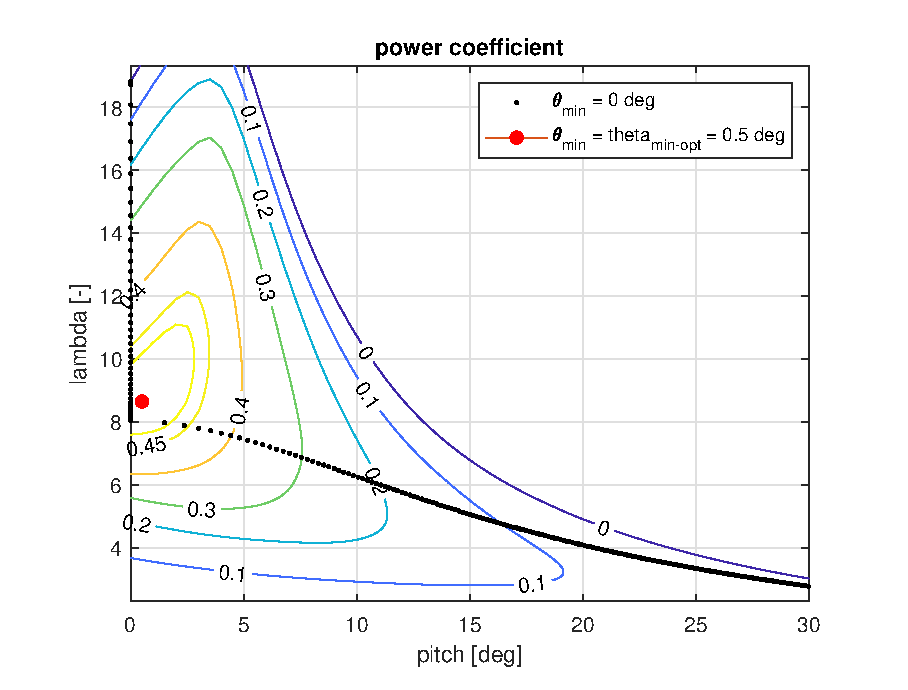
\includegraphics[width=12cm]{Figures/ThetaMinOpt}
	\caption{brute force optimization for minimum pitch angle $\theta$}
	\label{fig:theta min general}
\end{figure}

\section{Minimum Pitch Angle Optimization for Control Region 1.5 (Julius)} 
% !TEX spellcheck = en_US
% Theta min dynamic calculations
%=================================================================================
Since the control region 1.5 has a large wind speed range of \SI{3.28}{m/s} the optimization of the pitch angle could lead to an increase in AEP.
As optimization process a brute force approach was used in order to find the optimum pitch angle for every operating wind speed in region 1.5. 
During the calculation the pitch angle was optimized in a range of \SI{0}{\degree} to \SI{5}{\degree} with a step size of \SI{0.1}{\degree}. 
The results of the optimization can be seen in figure \ref{fig:theta min dynamic}. 
The result shows, that keeping a static pitch angle through region 1.5 is not leading to the optimal power production. 
A calculation of the AEP with a dynamic pitch adjustment for region 1.5 leads to an increase of \SI{0.19}{\%} compared to a static minimum pitch angle of \SI{0.5}{\degree} as shown in section \ref{minimum pitch angle static}.
(Calculated with Weibull parameters of TC III and $k=2$.)
Since the calculation is done without transition regions for the adjustment of the pitch the increase in AEP after implementation of the control behavior is to be expected less than the named \SI{0.19}{\%}.
The approach of changing the pitch angle dynamically in region 1.5 was not implemented in the OPTIMUS Shakti project but could be interesting for further optimization of the developed WT.  

\begin{figure}[h]
	\centering	
	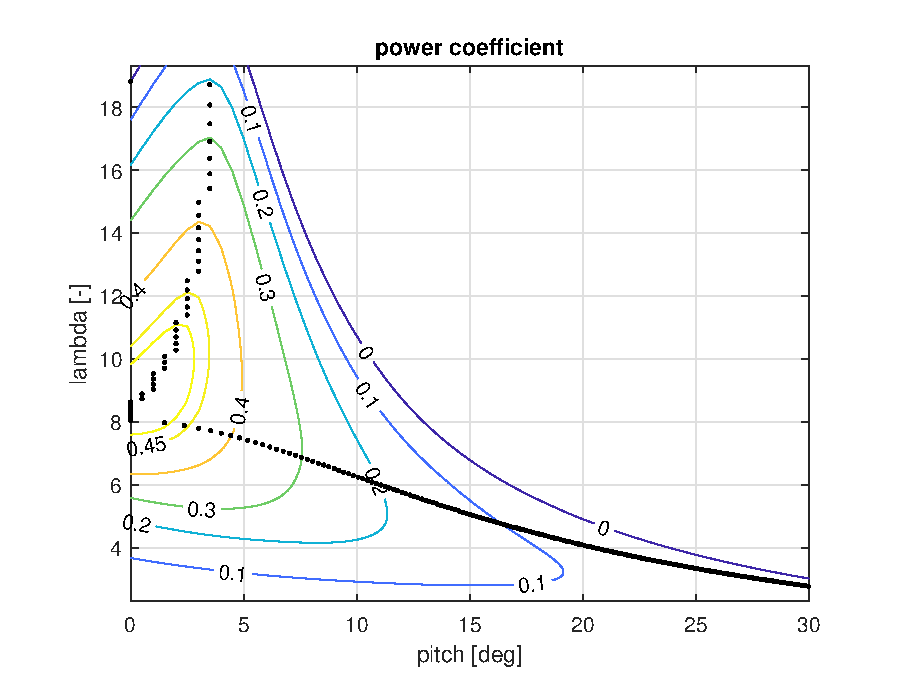
\includegraphics[width=12cm]{Figures/ThetaMinOptDynamic}
	\caption{brute force optimization for minimum pitch angle $\theta$ in region 1.5}
	\label{fig:theta min dynamic}
\end{figure}
